%! Author = noone
%! Date = 5/3/23

% Preamble
\documentclass[11pt]{article}

% Packages
\usepackage{amsmath}
\usepackage{blindtext}
\usepackage{amsfonts}
\usepackage{graphicx}

% Document
\title{Sections and Chapters}
\author{Overleaf}
\date{\today}

\begin{document}
\maketitle
\section{What is Regression analysis?}\label{sec:what-is-regression-analysis?}

Regression Analysis investigates the functional relationship between statistical variables.
Data are usually multiple observations of a random vector $(Y,x)$.
\begin{itemize}
\item $x=(X1,\dots,Xp)^T$ is a $p$-vector of variables termed: \underline{explanatory variables}, regressors, predictors, input variables or \underline{independent variables}.
\item $Y$ is called: response variable, target variable, output variable, outcome variable or dependent variable.
It may be continuous $(\in \mathbb{R})$, discrete $(\in \{1,\dots,K\} \in \{1,\dots,K\})$ or ordinal (ordered discrete).
\end{itemize}
Response variables are usually treated as \textbf{random variables}, while predictors are treated as \textbf{fixed observations}.
\blindtext

\section{Response and explanatory variables}\label{sec:response-and-explanatory-variables}
Response and explanatory variables

Response and explanatory variables are measures on one of the following scales:
\begin{itemize}
\item \textbf{nominal}: when $Y$ is classified into categories, which can be only two (binary outcome) or several (multinomial outcome)
\item \textbf{ordinal}: when $Y$ is recorded in classes
\item \textbf{continuous}: when $Y$ is measured on a continuous scale, at least in theory.
\end{itemize}
Nominal and ordinal data are discrete variables and can be \underline{qualitative} or \underline{quantitative} (eg \text{counts}).
Continuous data are \underline{quantitative}.
$x$ can also be quantitative or qualitative.
In particular, when the explanatory variable is \underline{qualitative}, it is often called factor.
A quantitative explanatory variables is called \underline{covariate}.
\blindtext

\section{Regression}\label{sec:Regression}
We aim to find a ``good'' functional relationship of the form $Y=f(x)+\epsilon Y = f(x) + \epsilon$, where $\epsilon$ is a random error term independent of $x$ with mean zero.
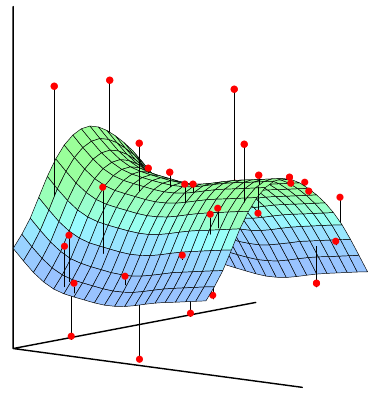
\includegraphics{images/figure-1-1-1}
\blindtext

\section{applied regression analysis}\label{sec:applied regression analysis}
Applied means: ``If there is no way to calculate it, we won't talk about it.''
On the other hand, we want to understand the underlying computational methods and algorithms.
This will be impossible without understanding the theory.
``There is nothing more practical than a good theory.''
— Kurt Lewin
\blindtext

\section{General Framework of statistical learning}\label{sec:General-framework-of-statistical-learning}
Statistical learning refers to a vast set of tools for understanding data.
It splits into supervised and unsupervised methods.
All the methods presented in this course are within the framework of supervised learning.
Regression fits into the framework of supervised methods, which requires a statistical model for predicting or estimating an output based on one or more inputs.

In contrast, unsupervised methods cover situations where there are inputs but no supervising output.
In these type of analysis we learn about relationships and structure of data.
Example of unsupervised analysis is cluster analysis.
\blindtext

\section{Knowledge Assumed}\label{sec:Knowledge-Assumed}
Knowledge assumed

You need to have a fairly good understanding of linear algebra:
\begin{itemize}
\item vector spaces.
\item linear independence.
\item matrix multiplication.
\item diagonalisation.
\item projections.
\end{itemize}

Need to know multivariate calculus:
\begin{itemize}
\item partial derivatives,
\item critical points,
\item integrals,
\end{itemize}

It's also good to have some previous exposure to computational software (RR):
\begin{itemize}
\item data types,
\item manipulation of arrays,
\item some idea of optimisation,
\end{itemize}

And finally, you need to know some probability theory and statistics:
\begin{itemize}
\item important distributions (normal, Poisson),
\item conditional probability,
\item conditional expectation,
\item covariance matrix,
\item asymptotic normality of maximum likelihood estimators,
\end{itemize}
\blindtext

\end{document}
